\documentclass[tikz, border=5pt]{standalone}
\usepackage{array, flowchart}

\usetikzlibrary{arrows.meta, calc, chains, quotes, positioning, shapes.geometric}
\tikzset{FlowChart/.style={
    node distance = 5mm and 10mm,
    start chain = A going right,
    base/.style = {draw, minimum width=16mm, minimum height=19mm, align=center, on chain=A, text width=4cm},
    process/.style = {base},
    rounded/.style = {base, rounded corners},
    every edge quotes/.style = {auto=right}
}}

\begin{document}
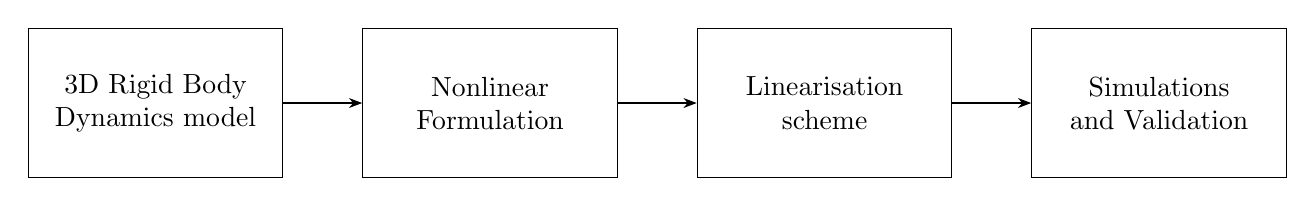
\begin{tikzpicture}[FlowChart]
    \node [process, text width=3cm] {
        3D Rigid Body Dynamics model
    };
    \node [process, text width=3cm] {
        Nonlinear Formulation
    };
    \node [process, text width=3cm] {
        Linearisation scheme
    };
    \node [process, text width=3cm] {
        Simulations and Validation
    };

    \draw [arrows=-Stealth]
    (A-1) edge (A-2)
    (A-2) edge (A-3)
    (A-3) edge (A-4);
\end{tikzpicture}
\end{document}
